\subsection{Processor overview}

The processor described in this report is a pipeline consisting of five stages:
PC handling, instruction decoding, executing, memory and write-back. Each stage
is described closely in the following subsections. In addition to the stages, 
there is a control unit and multiple hazard- and error-detecting and -handling units. 
These are also described in the following subsections. The architecture overview is 
shown in figure~\ref{fig:processor}. The figure also shows the connections to the 
framework supplied in the assignment, and memory access. To keep the figure readable, where these input and output signals are connected within the processor were omitted. Each stage is also shown as a blackbox.

\begin{figure}[ht]
        \centerline{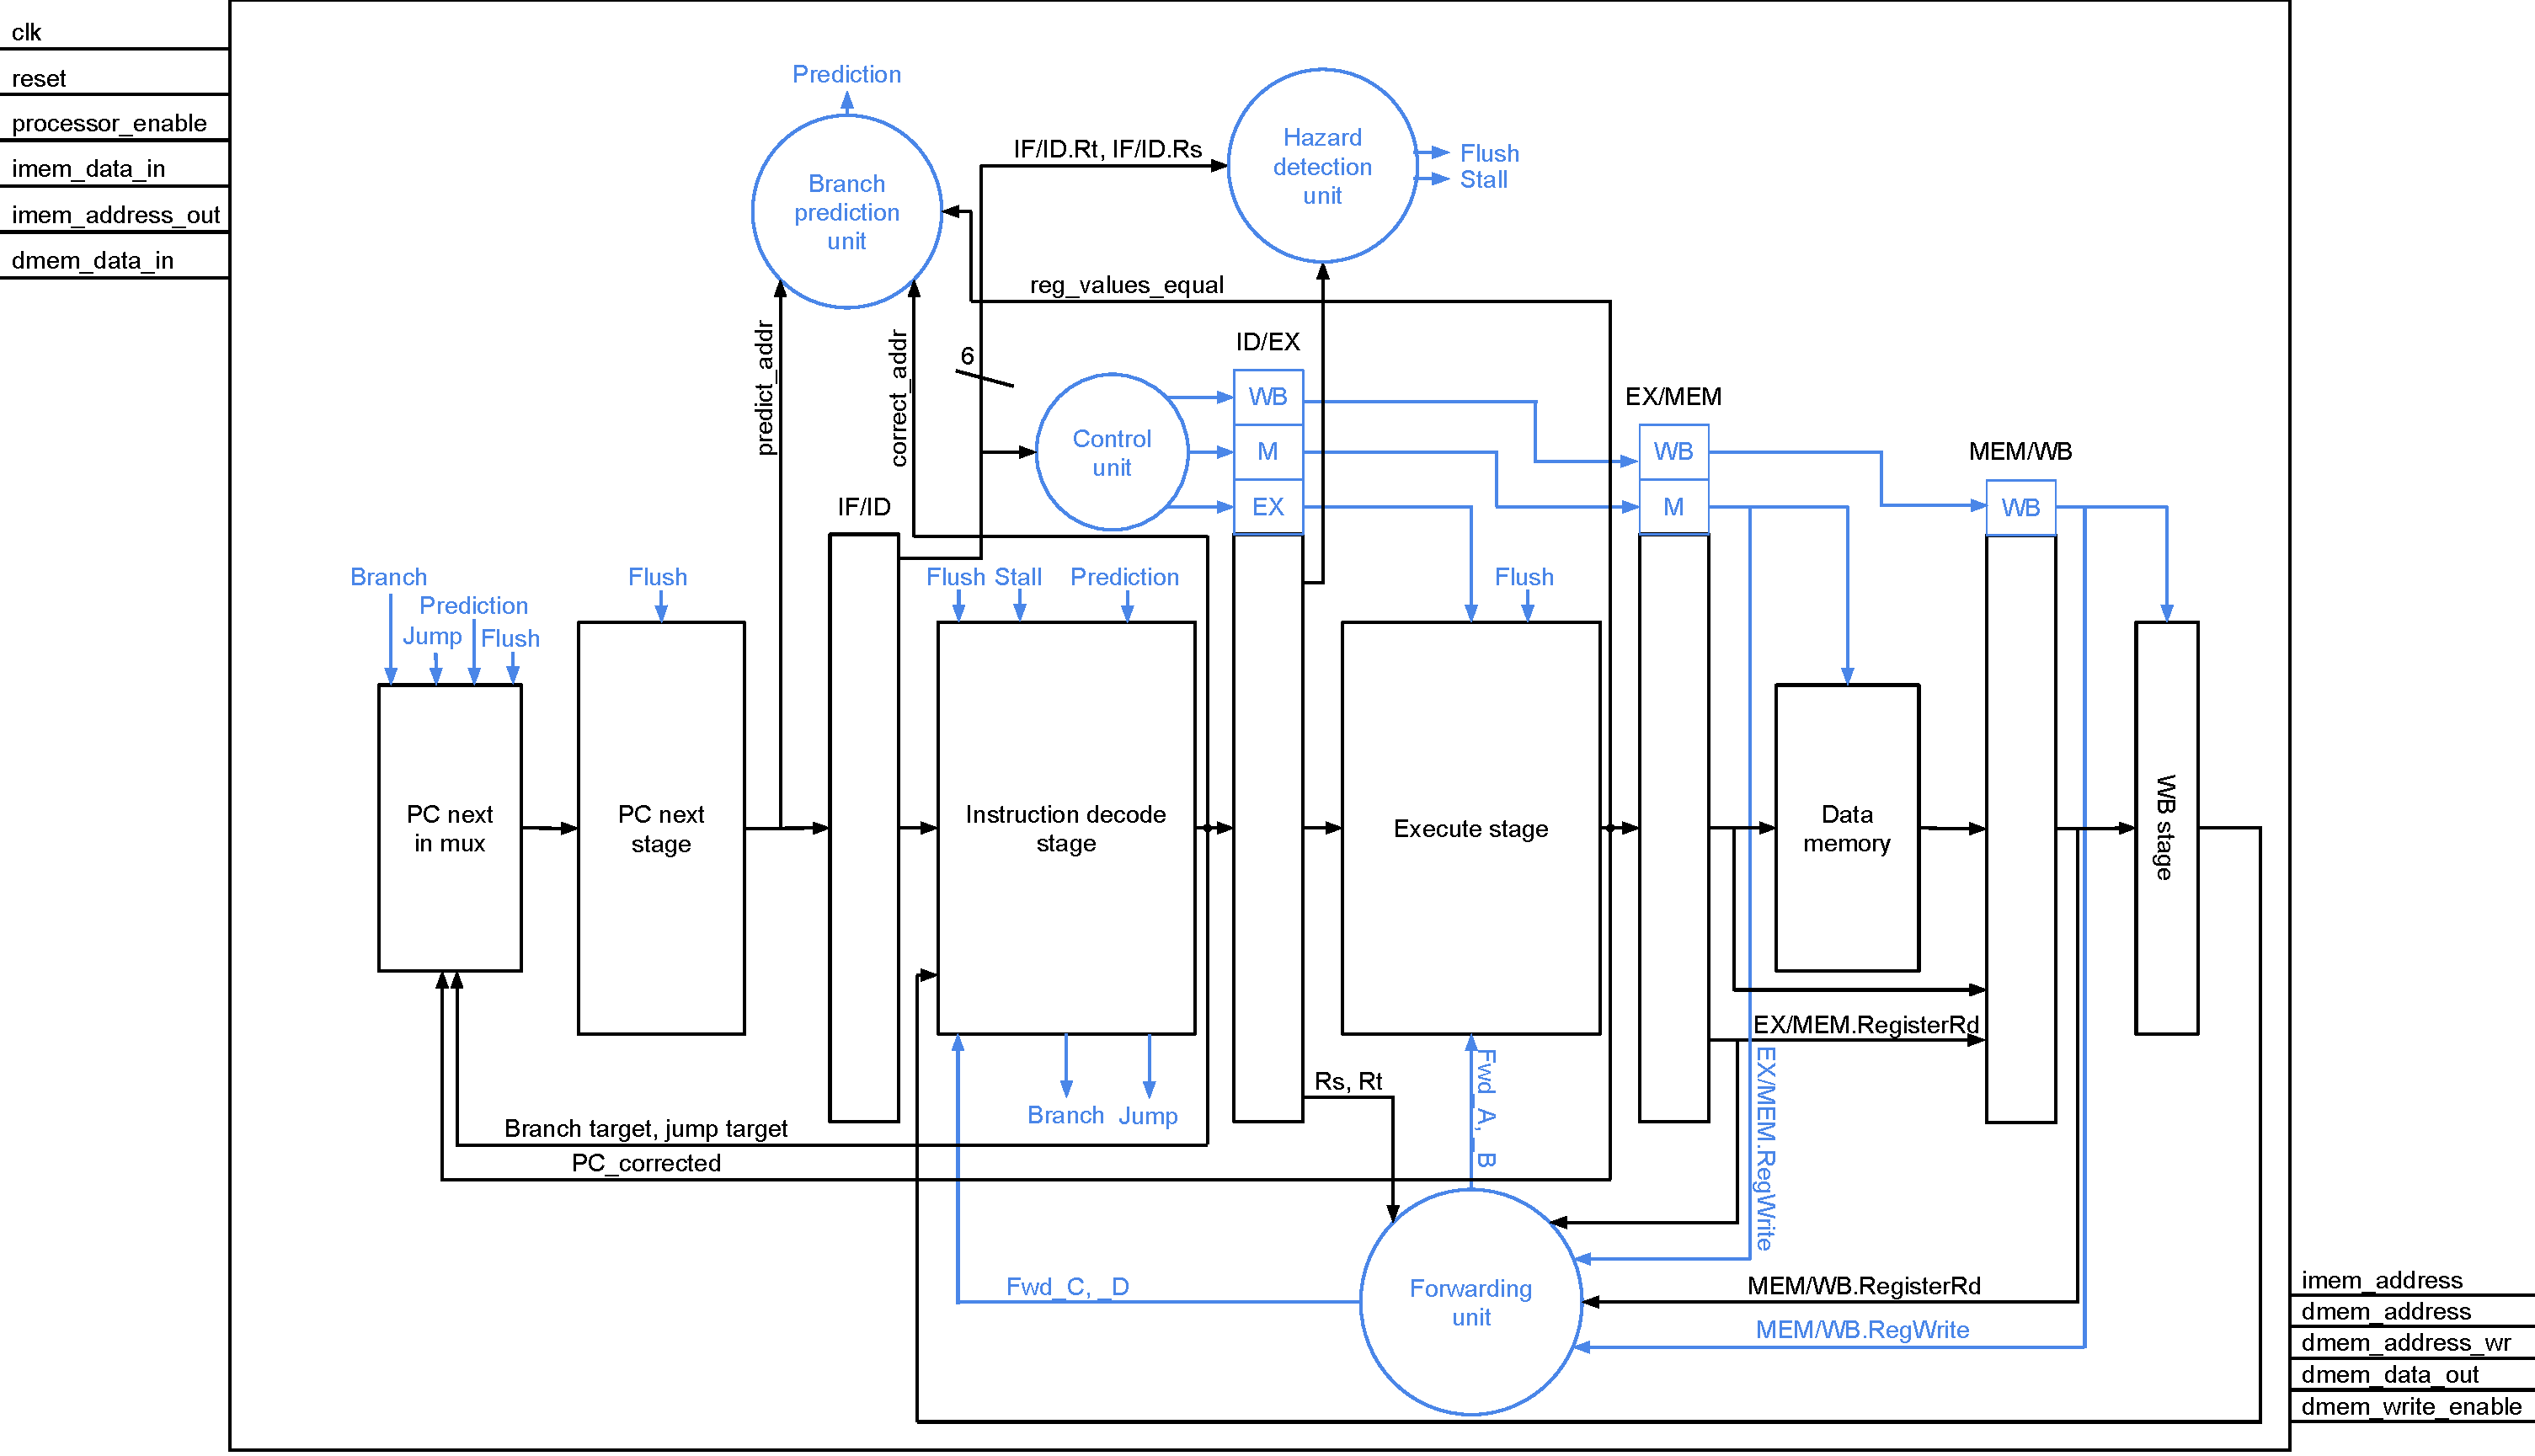
\includegraphics[width=500px]{figures/processor_arch}}
        \caption{Processor overview  - how the stages and conrtol units are connected}
        \label{fig:processor}
\end{figure}

In theory we wanted a clean separation of the stages and the different units,
and as a result to only have connections and no logic on the processor level of the implementation.
In practice this separation turned out not to be as clean as intially planned
and we ended up with a little bit of logic implemented on the processor level.

Most notably the processor contains a pc next mux, this happend because 
all branching and jump decisions initially took place in the execute stage. As we iterated the 
design, implementing eager jumping and predictive branching, pc decisicions happen
in both the id and execute stages, and the choice was made to move the pc next mux up one level.
The only viable alternative would have been to extend the number of input signals to the 
pc next stage, and have the mux there, but we felt that both alternatives would result
in an equal amount of complexity.

The memory stage theoretically only contains the memory file. As memory in our design
is external, this stage is only wiring, and these wires are implemented at the 
processor level. This solution was less complex than extracting this to a separate
stage file.

The different external units take their input from the pipeline stages. Instead
of adding extra outputs to the stages to accomodate the required inputs on the
different units, we opted for connecting the units directly to the output port of the
corresponding pipeline register when possible. 

All the these choices were made to reduce the number of signals needed at the processor level,
at the cost of a slightly less reabable component.


